\section{Arrows}
\begin{center}
	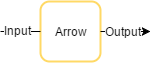
\includegraphics[]{images/arrow.png}
\end{center}
Arrows were introduced by Hughes \citHughes ~as a general interface for computation. An arrow \code{arr a b} can be look at as a computation that converts an input \code{a} to an output \code{b}. This is defined in the arrow typeclass:

\begin{minipage}{\textwidth}
\begin{minipage}{0.5\textwidth}
\begin{lstlisting}[frame=htrbl]
class Arrow arr where
arr :: (a -> b) -> arr a b



(>>>) :: arr a b -> arr b c -> arr a c




first :: arr a b -> arr (a,c) (b,c)
\end{lstlisting}
\end{minipage}
~~~~
\begin{minipage}{0.25\textwidth}
	~\\~\\~\\
	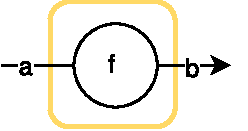
\includegraphics[scale=0.6]{images/arr}~\\~\\
	\includegraphics[scale=0.6]{images/compose}~\\~\\
	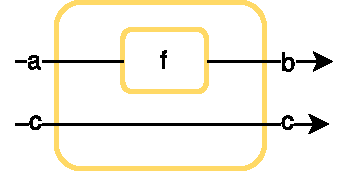
\includegraphics[scale=0.6]{images/first}~\\~\\
\end{minipage}
\end{minipage}
\lstinline{arr} is used to lift an ordinary function to an arrow type. This can be thought of as analogous to the monadic \lstinline{return}. The \lstinline{>>>} operator, in a similar way, is analogous to the monadic composition operator \lstinline{>>=} and combines two arrows \code{arr a b} and \code{arr b c} by "wiring" the outputs of the first to the inputs to the second to get a new arrow \code{arr a c}. And lastly, the \lstinline{first} operator, which takes the input arrow from b to c and converts it into an arrow on pairs with the second argument untouched, is also needed for actual useful code as without it, we wouldn't have a way to save input across arrows.
\\\\
The most prominent instances of this interface are regular functions \lstinline{(->)},
\begin{lstlisting}[frame=htrbl]
instance Arrow (->) where
	arr f = f
	f >>> g = g . f
	first f = \(a, c) -> (f a, c) 
\end{lstlisting}
and the Kleisli type
\begin{lstlisting}[frame=htrbl]
data Kleisli m a b = Kleisli { run :: a -> m b }
\end{lstlisting}
as well:
\begin{lstlisting}[frame=htrbl]
instance Monad m => Arrow (Kleisli m) where
	arr f = Kleisli $ return . f
	f >>> g = Kleisli $ \a -> f a >>= g
	first f = Kleisli $ \(a,c) -> f a >>= \b -> return (b,c)
\end{lstlisting}
\begin{figure}
	\centering
	\begin{tabular}{cc}
		\subcaptionbox{first\label{1}}{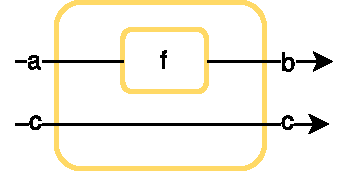
\includegraphics[width = 1.5in]{images/first}} &
		\subcaptionbox{second\label{2}}{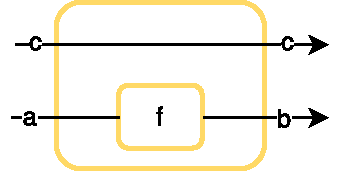
\includegraphics[width = 1.5in]{images/second}} \\
		\subcaptionbox{(***)\label{1}}{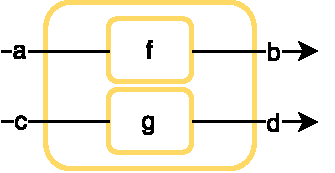
\includegraphics[width = 1.5in]{images/starstarstar}} &
		\subcaptionbox{(\&\&\&)\label{2}}{\includegraphics[width = 1.5in]{images/andandand}}\
	\end{tabular}
	\caption{syntactic sugar}
	\label{3}
\end{figure}
With this typeclass in place, Hughes also defined some syntactic sugar: The mirrored version of \lstinline{first}, called \lstinline{second},
\begin{lstlisting}[frame=htrbl]
second :: Arrow arr => arr a b -> arr (c, a) (c, b)
second f = arr swap >>> first f >>> arr swap
	where swap (x, y) = (y, x)
\end{lstlisting}
the *** combinator which combines first and second to handle two inputs in one arrow,
\begin{lstlisting}[frame=htrbl]
(***) :: Arrow arr => arr a b -> arr c d -> arr (a, c) (b, d)
f *** g = first f >>> second g
\end{lstlisting}
and the \&\&\& combinator that constructs an arrow which outputs 2 different values like ***, but takes only one input.
\begin{lstlisting}[frame=htrbl]
(&&&) :: Arrow arr => arr a b -> arr a c -> a a (b, c)
f &&& g = arr (\a -> (a, a)) >>> (f *** g)
\end{lstlisting}
A short example given by Hughes on how to use this is \lstinline{add} over arrows:
\begin{lstlisting}[frame=htrbl]
add :: Arrow arr => arr a Int -> arr a Int -> arr a Int
add f g = (f &&& g) >>> arr (\(u, v) -> u + v)
\end{lstlisting}
The benefit of using the \code{Arrow} typeclass is that any type which is shown to be an arrow can be used in conjunction with this newly created \lstinline{add} combinator. Even though this example is quite simple, the power of the arrow interface immediately is clear: If a type is an arrow, it can automatically used together with every library that works on arrows. Compared to simple monads, this enables us to write code that is more extensible, without touching the internals of the specific arrows.
\\\\
\textit{Note: In the definitions Hughes gave in his paper, the notation \code{a b c} for an arrow from \code{b} to \code{c} is used. We use the equivalent definition \code{arr a b} for an arrow from \code{a} to \code{b} instead, to make it easier to find the arrow type in type signatures.}